\documentclass{article}

\title{全能力排样}
\subtitle{从语法到页面的每一项能力，都放在同一份文档里}
\author{soma-typeset}
\date{2026-11-26}
\language{zh-Hans}
\colophon{soma-typeset · 全能力样张 · 2026 · Apache-2.0}

\newcommand{\engine}{\textsf{soma-typeset}}
\newcommand{\term}[2]{\textbf{#1}（#2）}
\newcounter{demo}

\begin{document}

\section{文本、强调与行内对象}

这一段用来检查正文的基本形态：首行缩进两字，两端对齐，中文与 Latin 混排时由规则层插入 CJK/Latin 间隙，而不是靠作者敲空格。标点按禁则处理——行首不出现句号与逗号，行尾的左括号会被推到下一行；行边在超宽时裁掉标点的侧空，而不是压扁字面。\engine{} 把这些都放在规则表里，断行器只认宽度。

行边裁剪只发生在行的两端：行尾的句号与逗号在两端对齐的行上总会让出侧空；行首的左引号与左括号在两端对齐行、以及标题/左对齐行的行首都会贴墨对齐，只有其他普通字符的行首侧空留给超宽救援。挤压量来自字体真实的墨迹边界，而不是猜出来的常数；换一张脸，裁剪量随之改变，断点却由字符类别与标点决定，不由作者按没按快捷键决定。

强调是源文档的事实：\textbf{加粗}、\emph{斜体}、\underline{下划线}、\textsc{Small Caps}、\textsuperscript{上标}、\textsubscript{下标}，以及不可断的等宽对象 \texttt{soma.render/7}。链接只画文字，PDF 里是真正的 \href{https://example.com/soma}{注解矩形}；URL 只在斜杠与点后给出断点，字母中间不会被截断，例如 \url{https://example.com/a/very/long/path/that/must/not/be/split}。

中文里嵌公式也是行内对象：质量与能量满足 $E = mc^2$，水的分子式是 $H_2O$，平方和 $x^2 + y^2 = r^2$。行盒会因为公式的上下伸而变高，后续行随之让位；公式的宽度来自它自己的盒子，而不是它占了多少个字符。

注音是另一类行内对象：\ruby{排版}{pái bǎn} 与 \ruby{汉字}{hàn zì} 的读音落在基字正上方，基字保持一个原子，注音不会与上一行的降部相撞。行盒会为注音向上多留出半行；同一页里没有注音的行不受影响。

\section{结构：列表、引文与代码}

结构层只描述“这是什么”，不描述“长什么样”。列表的记号在文字列左侧，续行回到文字列，这是悬挂缩进而不是整条缩进；列表可以嵌套，也可以包含段落、公式与代码。等宽块不做断行，也不做首行缩进；超宽时宁可在行尾溢出，也不在命令中间插入换行——复制出去的必须是能跑的命令。

\begin{verbatim}
cargo run -p soma-cli -- render \
  --input full.tex --template full.yaml \
  --metrics full.smt --hyphenation hyphen-en.pat \
  --format pdf --out full.pdf
\end{verbatim}

无序列表的记号是圆点，重点在续行的对齐：

\begin{itemize}
\item 第一层：断行是全局最优，代价函数由每行的松紧、固定行数、标点挤压量、中英边界偏差与末行长短相加而成。
\item 第一层：每一项都能单独标定、单独解释。
  \begin{itemize}
  \item 第二层：标点禁则与行边裁剪是规则，不是常数。
  \item 第二层：规则表带版本号，改规则就换哈希。
    \begin{itemize}
    \item 第三层：三层以后不再缩进，避免文字列被挤成窄条。
    \end{itemize}
  \end{itemize}
\item 第一层：列表可以包含段落、公式与代码。
\end{itemize}

有序列表保留起始编号。编号是列表的事实，不是模板的装饰：从 3 开始的有序列表，第一项就写 3：

\begin{enumerate}
\item 先编译 DocIR，语法前端只产出结构。
\item 再把 DocIR 与模板合成为盒子树。
\item 最后断行、分页并输出页面结果。
\end{enumerate}

\term{描述列表}{description} 的记号是词，不是圆点；词后面跟一个全角空格，然后才是释义：

\begin{description}
\item[断行] 在段落内寻找全局代价最小的断点序列。
\item[分页] 在页面高度上做同样的优化，脚注计入页面开销。
\item[度量] 一张整数表，记录每个字的前进宽度与上下伸。
\end{description}

引文左右缩进，不重复首行缩进。缩进本身就是“这是另一个声音”的信号，再叠一个首行缩进只会让读者以为是正文：

\begin{quote}
排版不是把字摆整齐，而是让读者在每一行的末尾不必停顿。行末出现一个孤零零的标点，读者会先看到它，再回头找它所属的句子——这一瞬间的迟疑，就是坏版面的全部代价。
\end{quote}

引文结束后回到正文，缩进与行距都恢复。结构层不记录“引文用了多宽的缩进”，那是模板的事；同一份文档换模板，缩进可以完全不同，而 DocIR 一个字节都不用改。

\section{表格、图片与题注}

表格的列宽按内容分配，不按列数平分：一个“序号 / 说明”的表格不会把版心各分一半。跨列单元格按列宽之和占位，跨行单元格让所在行带变高，后续行依次顺延；表头在续页重复，续页的第一条横线与首页一致。

\begin{table}
\caption{能力清单的一角}
\begin{tabular}{lll}
\hline
层面 & 能力 & 状态 \\
\hline
语法 & Markdown / HTML / LaTeX / Word & 已接 \\
\multicolumn{3}{l}{排版：断行、分页、脚注、索引} \\
结构 & 表格、图片、公式、注音 & 已接 \\
\hline
\end{tabular}
\end{table}

题注在表的上方、图的下方，编号由模板生成。题注本身也是可断行的段落：一行放不下就换行，而不是缩字号；图目录与表目录里的页码来自第二遍排版，与正文页码同时收敛。

图片的盒子尺寸来自位图自身的宽高比，PNG 走无损路径，JPEG 直通阅读器。两张图并排会互相挤压，所以这里一上一下，各占一条版心宽度：

\begin{figure}
\centering
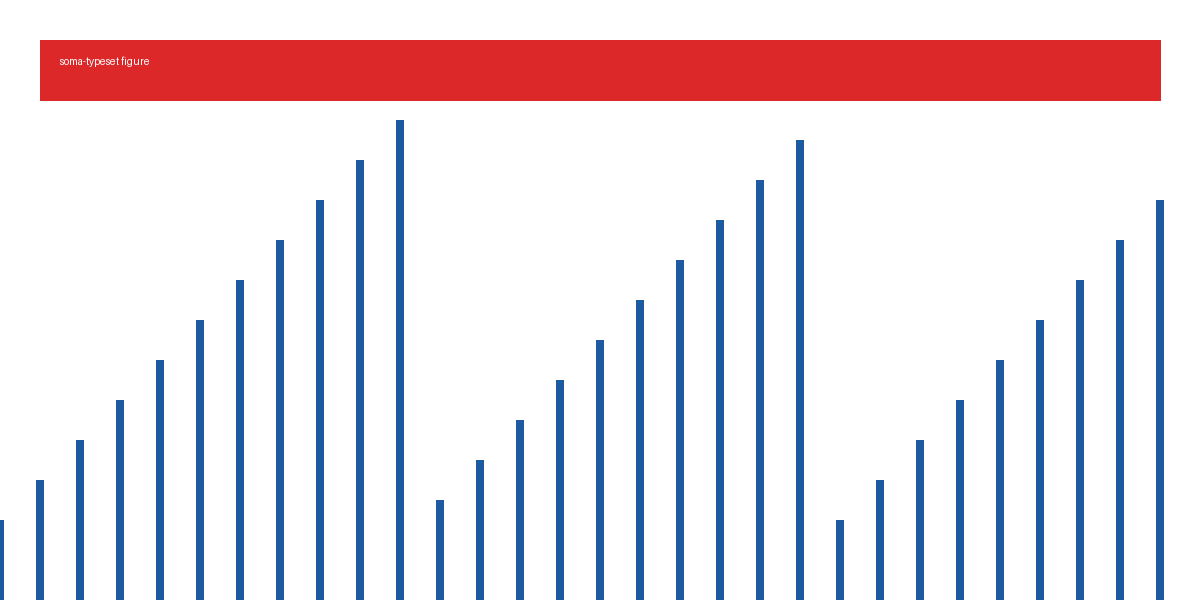
\includegraphics{fig/pipeline.png}
\caption{一张 PNG 位图：像素由后端解码后重新压缩}
\end{figure}

\begin{figure}
\centering
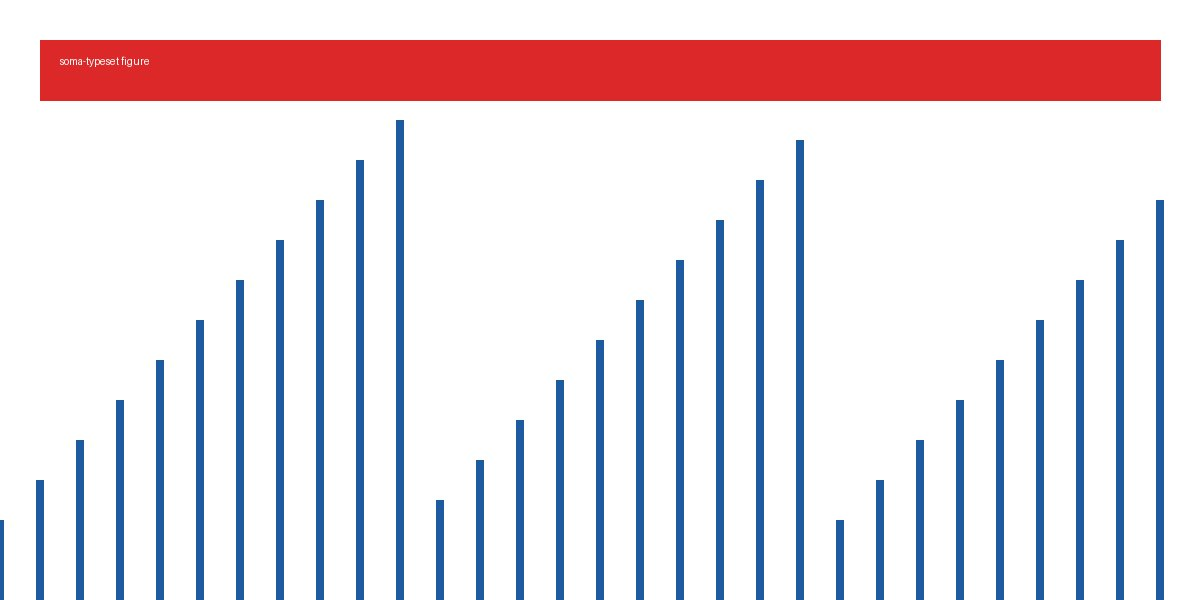
\includegraphics{fig/photo.jpg}
\caption{一张 JPEG 位图：原样嵌入，由阅读器解码}
\end{figure}

图与图之间留出一行的空隙，避免两张图在视觉上粘成一张；图题与下一段之间同样留白，读者不会把图题误读成下一段的开头。

\section{公式、宏与计数器}

显示公式单独成块，居中，上下留白。求和号在显示样式下把上下限排在符号上下；分式与根号各有自己的几何，分数线是真实的矩形，根号的横线压在被开方数上方：

\[
\sum_{i=1}^{n} a_i x^i \qquad \frac{\sqrt{\pi}}{2}
\]

array 的列格式控制对齐；\substack{} 把两个下标堆成两行；变量按数学习惯排成斜体，函数名与文字模式保持正体：

\[
\begin{array}{lcr}
\text{left} & \text{mid} & \text{right} \\
1 & 22 & 333
\end{array}
\qquad
\sum_{\substack{i=1\\j=1}}^{n} a_{ij}
\]

需要编号的公式用 equation 环境；多行的 align 按 \& 对齐，每行各自编号。\tag 换成自己的号，\notag 让这一行不占号——两者都不消耗自动编号：

\begin{equation}
a^2 + b^2 = c^2
\end{equation}

\begin{align}
f(x) &= x^2 + 2x + 1 \\
g(x) &= \sqrt{x} \notag \\
h(x) &= \frac{1}{1+x} \tag{A}
\end{align}

宏在解析前展开，定义本身不进入版面。下面这句话用的是 \term{宏}{带两个参数}，引擎名是 \engine{}；宏体里可以再调用别的宏，展开深度有上限，写错也不会把整篇文档卡死。

\stepcounter{demo}\stepcounter{demo}\stepcounter{demo}

这是第 \arabic{demo} 步；换成罗马数字是 \roman{demo}，字母是 \alph{demo}。计数器只在本文档内有效，不会泄漏给模板的章节编号——模板生成的编号是另一套，两者互不干扰。

\section{断词}

英文长词在模式集允许的位置断开，断行时连字符的宽度计入行宽，所以两端对齐的行仍然停在版心边缘，而不是多出一个连字符。模式集由宿主提供，仓库不自带词典：换语言就换一张表，不用重新编译引擎。

模式只决定“哪里可以断”，不决定“一定断”。断点带一个低于行代价的惩罚，只有当整行找不到更好的断点、或者留下的空档会让 badness 明显变大时，断行器才会选择拆词。拆词点两侧至少要留两个与三个字母，缩写与全大写词不参与，URL、路径与邮箱地址也不参与——拆开一个地址，读者就无法复制。

A line of English prose is set here so that a long word such as internationalization can break at one of its pattern points instead of forcing an overfull line or a very loose one. 下一行继续用中文说明：连字符由渲染器画在行尾，它的宽度已经计进这一行，所以行尾不会越过版心。

连字符是断行的结果，不是源文档的字符：同一段文字换一个版心宽度，断点会移动，连字符也跟着移动；DocIR 与 canonical JSON 只记录“这一行在哪个边界断开”，不记录画了几个字符。

\section{脚注与索引}

脚注\footnote{脚注的高度反过来影响页面可用空间，因此必须与正文一起求解；这里的脚注里也有一个词条\index{脚注词条}，索引会把它记在引用所在页。}改变页面剩余空间：同一页里多一条脚注，正文就少一行，分页点也随之移动。所以脚注不是“排完正文再补”，而是和正文一起解的未知量；过高的一条脚注会把正文挤到下一页，而不是自己从中间断开。

索引在文末汇总，标记写在正文里。宋体\index{宋体}、表格\index{表格}、汉字\index{汉字}与字形\index{汉字!字形}都做了标记；排版\index{排版|seealso{汉字}}既有正文页码，也指向相关词条；旧称\index{旧称|see{汉字}}只有一条交叉引用，不再单独列出页码。索引的排序是模板的决定：这里用拼音，换一份模板可以改成码位。

拼音排序不是逐字查字典：每个汉字映射到一个无声调的音节排名，词条按“是不是汉字、音节排名、码位”逐字比较，拉丁字母与数字排在汉字之前。这样“八”不会排在“阿”前面，同音词也有稳定的先后。

索引词条支持两级以上：\texttt{汉字!字形} 是“汉字”下面的子条目，父条目没有单独标记时也会自动补一行；页码合并时连续三页以上写成起止页，两页仍然分开列，因为两页的区间省不下多少空间。

\section{索引与页码区间}

这一章与上一章一起演示页码区间：同一个词条连续出现在多页上，索引里应合并成“起—止”，而不是把每一页都列出来。合并只作用于阿拉伯数字页码，罗马页码与混合页码不合并；合并发生在索引生成阶段，不影响正文的分页，也不改变任何一页的页码。\index{页码区间}

页码区间的判定只看相邻两个标签的差值是否为 1。中间缺一页就断开，例如 3、4、6 会写成“3, 4, 6”而不是“3–6”；重复出现的同一页在合并前已经去重，所以“3、3、4”只会得到“3, 4”。这些规则都在索引模块里，和排序、see 引用共用同一份词条树。\index{页码区间}

区间是给读者省扫描时间的：看到“10–13”，读者知道这四个页面连续；看到“10, 11, 12, 13”，读者要逐个确认是不是连续。两页的区间反而更长，所以两页保持分开写：一个逗号比一个破折号少一个字符，也少一次判断。\index{页码区间}

索引生成在排版之后：先得到每一页的实际页码标签（前置页可能是罗马数字），再把标签按文档顺序拼成列表，最后做区间合并。页码标签可以是任意字符串，但只有能解析成整数的相邻标签才会合并。合并后的区间仍然是一个普通的索引行：左对齐的词条、引导点、右对齐的页码。\index{页码区间}

区间与交叉引用可以共存：一个词条既有连续的页码，又有“参见”目标时，页码在前、参见在后；只有“见”而没有页码的词条，不参与区间合并，因为它的作用是把读者送到别处，而不是列出讨论位置。\index{页码区间}

排序与区间是两件独立的事：先按拼音（或码位）把词条排好，再对每个词条的页码列表做一次线性扫描。排序改不了区间，区间也改不了排序；两者都在同一次索引生成里完成，输出是一棵扁平的、带层级的行列表。层级只影响缩进，不影响区间：父条目与子条目各自维护自己的页码列表，互不合并。\index{页码区间}

如果一份文档的词条只出现在一页上，就退化成单个页码，不带任何区间符号；如果只出现在相邻两页，就保留两个页码。规则简单，结果稳定，换一次排版只可能因为分页变化而移动，不会因为合并逻辑不同而改变写法。索引的标题也进入书签与页眉：它和章节标题一样，是一个可导航的目标；页码来自第二遍排版，与正文页码同时收敛。\index{页码区间}

区间写法还有一个边界：页码标签不一定是整数。前置页用罗马数字时，索引里可以出现“ii, iii”，但它们不会被合并成“ii–iii”——罗马数字的连续性是读者自己判断的，引擎不替读者猜。阿拉伯数字与罗马数字混排时同样不合并，避免把两种编号体系混成一段。\index{页码区间}

索引里的每个词条只保留一份页码列表，重复标记在同一页不会产生重复页码；跨页重复标记才会进入列表。因此“同一页里写三次”不会让索引变长，“三页各写一次”才会得到三个页码，再按连续性合并。\index{页码区间}

这些规则不依赖词条的文字，也不依赖排序方式：码位排序与拼音排序共用同一套页码合并，索引树的结构也共用同一套缩进。换排序只改变行的顺序，不改变某一行的内容。\index{页码区间}

页码合并的输入是“词条第一次出现的顺序”，输出是“读者看到的顺序”。两者不一定相同：文档里先写“排版”，后写“汉字”，索引按拼音排序后“汉字”在前。合并发生在排序之后，所以区间里的起止也按排好序的页码列表计算，而不是按正文顺序。\index{页码区间}

如果索引跨了前置页与正文页，同一词条可能同时有罗马页码与阿拉伯页码。引擎把它们都保留，但不跨体系合并：读者不会看到“ii–3”这种既不是罗马也不是阿拉伯的写法。\index{页码区间}

页码区间的实现只有一个线性扫描：相邻差值等于 1 就延长当前区间，否则收尾并开新段。没有回溯，没有二次排序，也没有按词条类型分叉；这就是为什么同一份文档重复排版，区间总是一样。\index{页码区间}

最后，区间也出现在目录与图目录的页码里吗？不。目录的每一行指向一个具体位置，页码必须精确；只有索引这种“同一主题散落在多处”的列表才需要区间。两类页码都来自同一次分页，但写法不同，这是内容性质决定的，不是实现偷懒。\index{页码区间}

索引的引导点与目录用的是同一套：词条在左、页码在右、中间是点。区别在于索引行可以缩进，而目录行按标题层级缩进；两者都不换行地重复点，点只画在最后一行。\index{页码区间}

页码列的宽度按四位数字预留，所以索引从 9 涨到 10、从 99 涨到 100 时，词条列不会整体重排。这也是排版稳定的一部分：同一份文档加一段内容，已有索引行的横向位置不该改变。\index{页码区间}

索引条目的文字可以带排序键：显示“排版”，按“paiban”排序；也可以带 see/see also。页码合并只处理页码，不处理文字；一个词条的文字在索引里只出现一次，页码列表挂在它下面。\index{页码区间}

\newpage

\section{数学排版附录}

这一节把常见公式放进同一份书籍版心，检查数学面、变量、根式、上下标与极限的实际效果。公式默认使用 New Computer Modern Math，与参考样张的数学面一致。

\subsection{分数与根式}

\[
\frac{a}{b}, \quad \sqrt{x}, \quad \sqrt[n]{x}
\]

\subsection{上下标}

\[
x^2, \quad x_i, \quad x_{i,j}^{2n}, \quad e^{-x^2}
\]

\subsection{求和、积分与极限}

\[
\sum_{i=1}^{n} i = \frac{n(n+1)}{2}
\]

\[
\int_{0}^{\infty} e^{-x^2} dx = \frac{\sqrt{\pi}}{2}
\]

\[
\lim_{x \to 0} \frac{\sin x}{x} = 1
\]

\[
\prod_{k=1}^{n} k = n!
\]

\subsection{矩阵、分段与符号}

\[
\left( \begin{matrix} a & b \\ c & d \end{matrix} \right)
\qquad
f(x) = \begin{cases} x^2, & x \ge 0 \\ -x, & x < 0 \end{cases}
\]

\[
\alpha, \beta, \gamma, \delta, \epsilon, \theta, \lambda, \mu, \pi, \sigma, \phi, \omega
\]

\[
\Delta, \Gamma, \Theta, \Lambda, \Pi, \Sigma, \Phi, \Omega
\]

\subsection{重音与装饰}

\[
\hat{x}, \quad \bar{x}, \quad \vec{v}, \quad \tilde{n}, \quad \overline{a+b}, \quad \binom{n}{k}
\]

编号公式、对齐与宏仍在第四章演示；这里只增加公式类型，不改变模板。

\end{document}
